\section{Experiments}
\begin{figure}
  \centering
  \begin{subfigure}[b]{0.48\linewidth}
    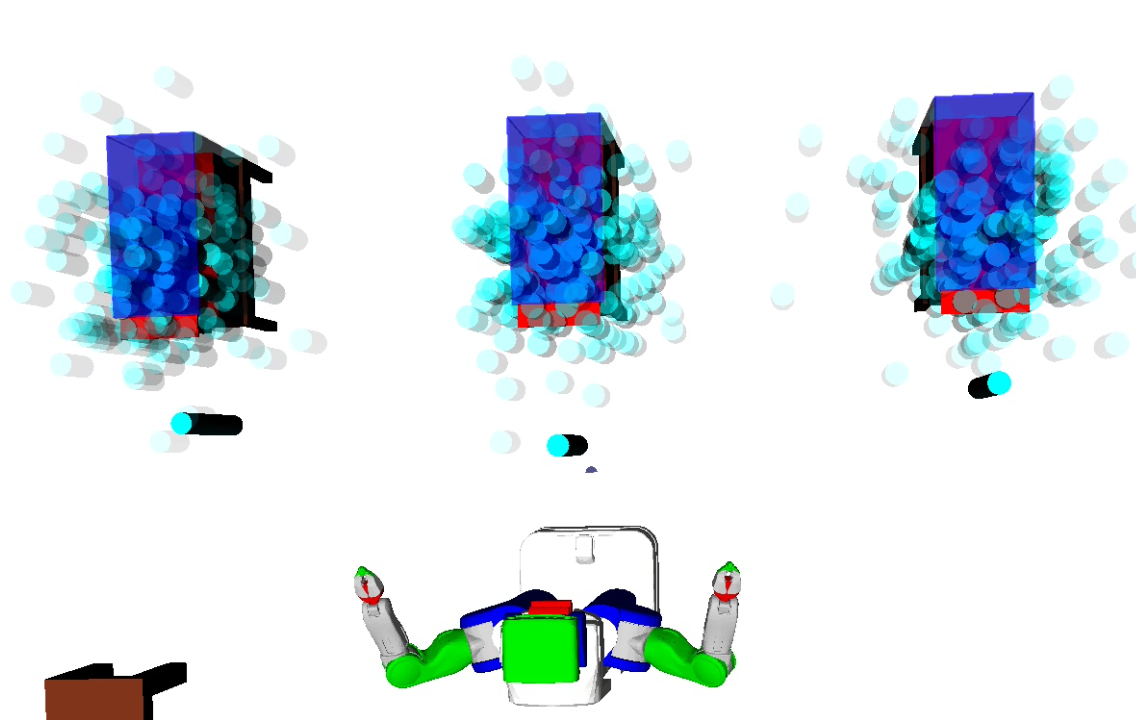
\includegraphics[width=\textwidth]{drawer_images/drawer_dist_0.png}
    \caption{}
  \end{subfigure}
  \begin{subfigure}[b]{0.48\linewidth}
    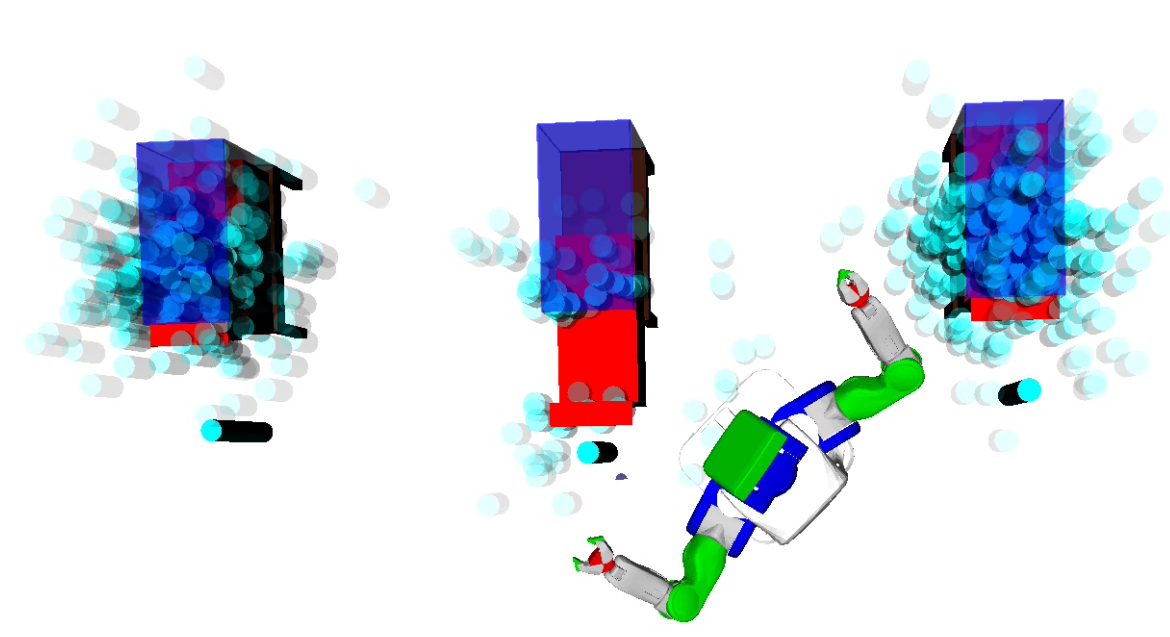
\includegraphics[width=\textwidth]{drawer_images/drawer_dist_1.png}
    \caption{}
  \end{subfigure}
  \begin{subfigure}[b]{0.48\linewidth}
    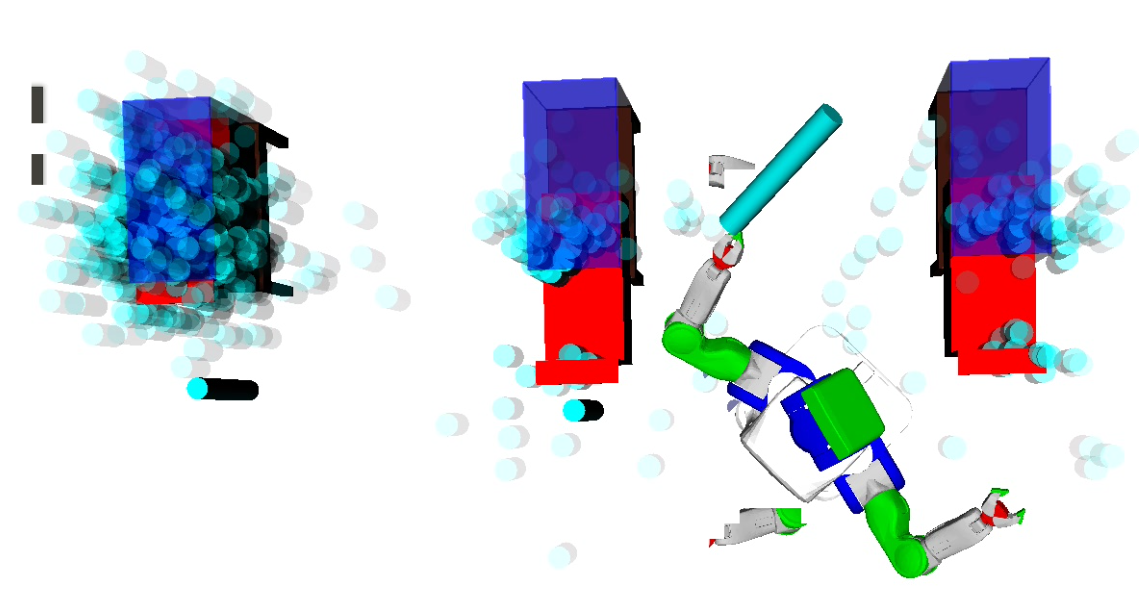
\includegraphics[width=\textwidth]{drawer_images/drawer_dist_2.png}
    \caption{}
  \end{subfigure}
  \begin{subfigure}[b]{0.48\linewidth}
    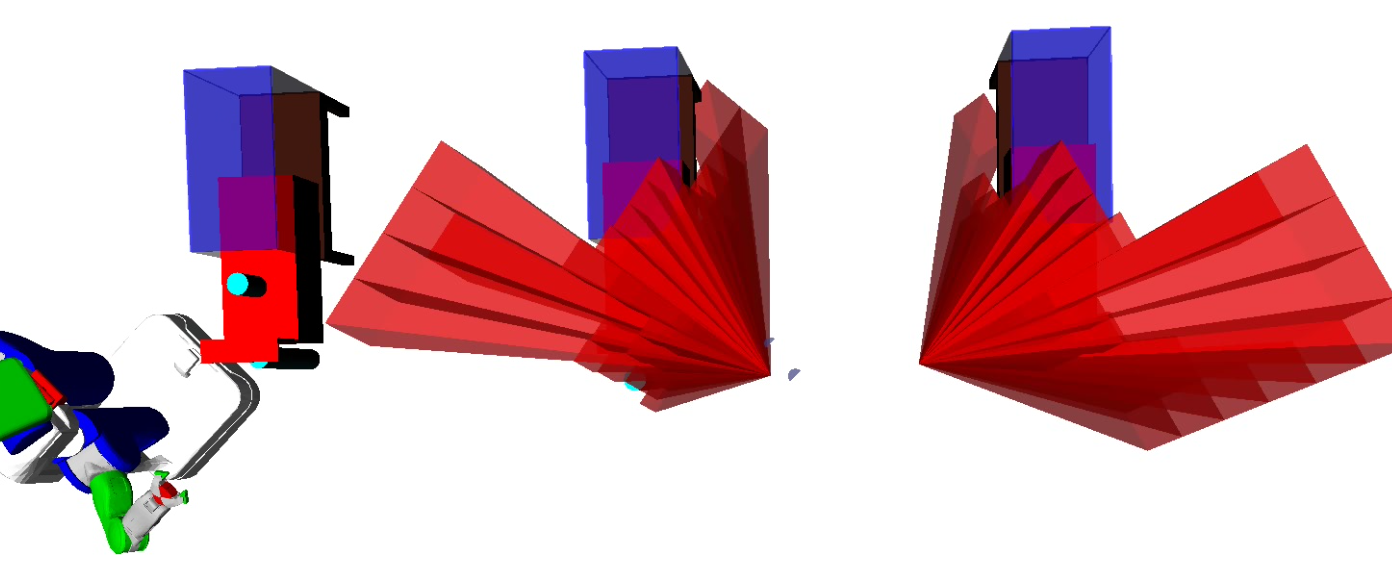
\includegraphics[width=\textwidth]{drawer_images/drawer_dist_negreg.png}
    \caption{}
  \end{subfigure}
  %% \begin{subfigure}[b]{0.3\linewidth}
  %%   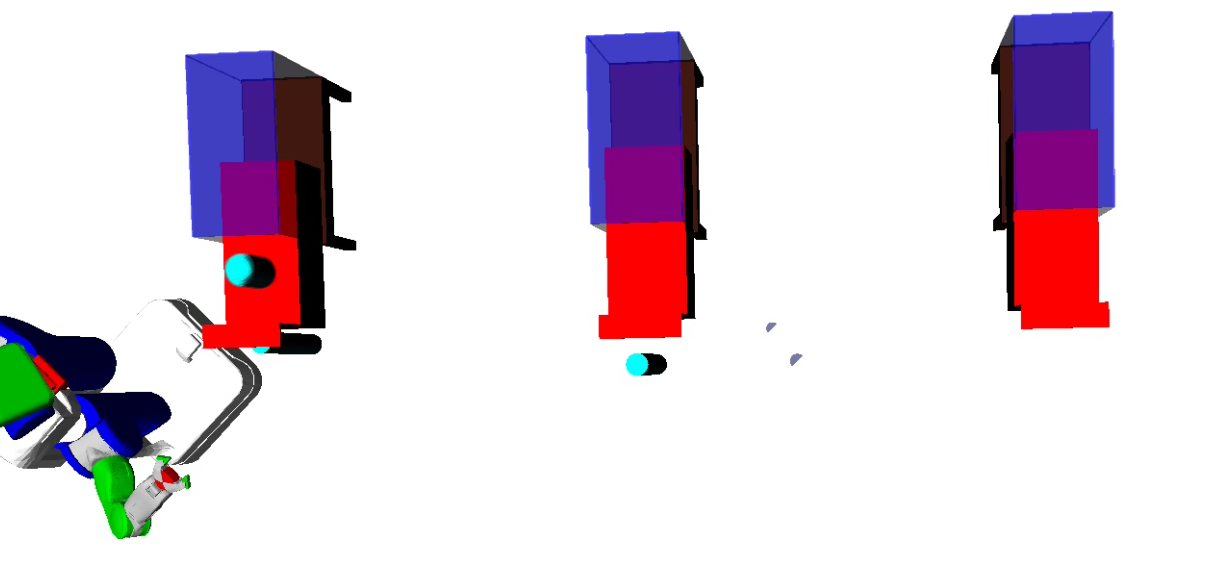
\includegraphics[width=\textwidth]{drawer_images/drawer_dist_3.png}
  %%   \caption{After observing three drawers (object was seen)}
  %% \end{subfigure}
  \caption{Intermediate belief states from a sample execution in our
    drawer search domain. The robot is initialized with a mixture of
    Gaussians distribution that places the object in one of three
    drawers. Beliefs are illustrated with samples from the posterior
    distribution and likelihoods are indicated by the level of
    transparency. In this run, the object was in the leftmost drawer
    and was found after searching the other drawers because they had a
    higher likelihood of containing the object. (a) shows the initial
    belief. (b) and (c) show intermediate states where \ibsp{}
    replanned after receiving an observation that indicated its
    current plan would fail. Notice that we only clear the obstruction
    in front of the drawer when it prevents opening the drawer far
    enough to observe the object. (d) shows the view cones from
    negative observations that were generated during planning.}
  \label{fig:drawerimgs}
\end{figure}

\begin{figure*}
  \centering
  \begin{subfigure}[b]{0.22\linewidth}
    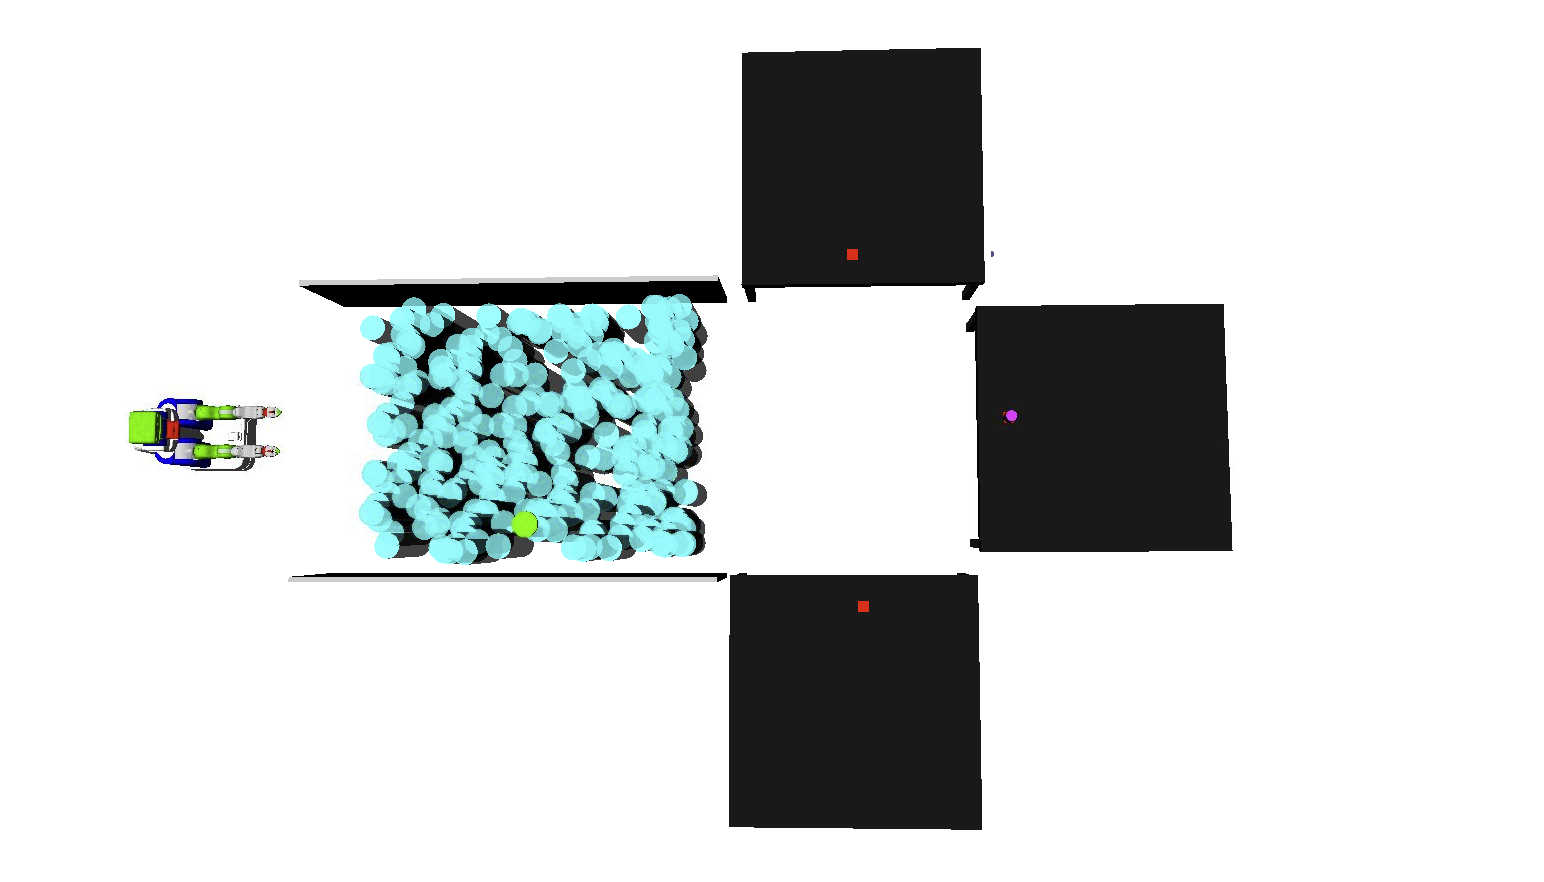
\includegraphics[width=\textwidth]{corridor_images/0-observe.png}
    \caption{Initial belief state}
  \end{subfigure}
  \begin{subfigure}[b]{0.22\linewidth}
    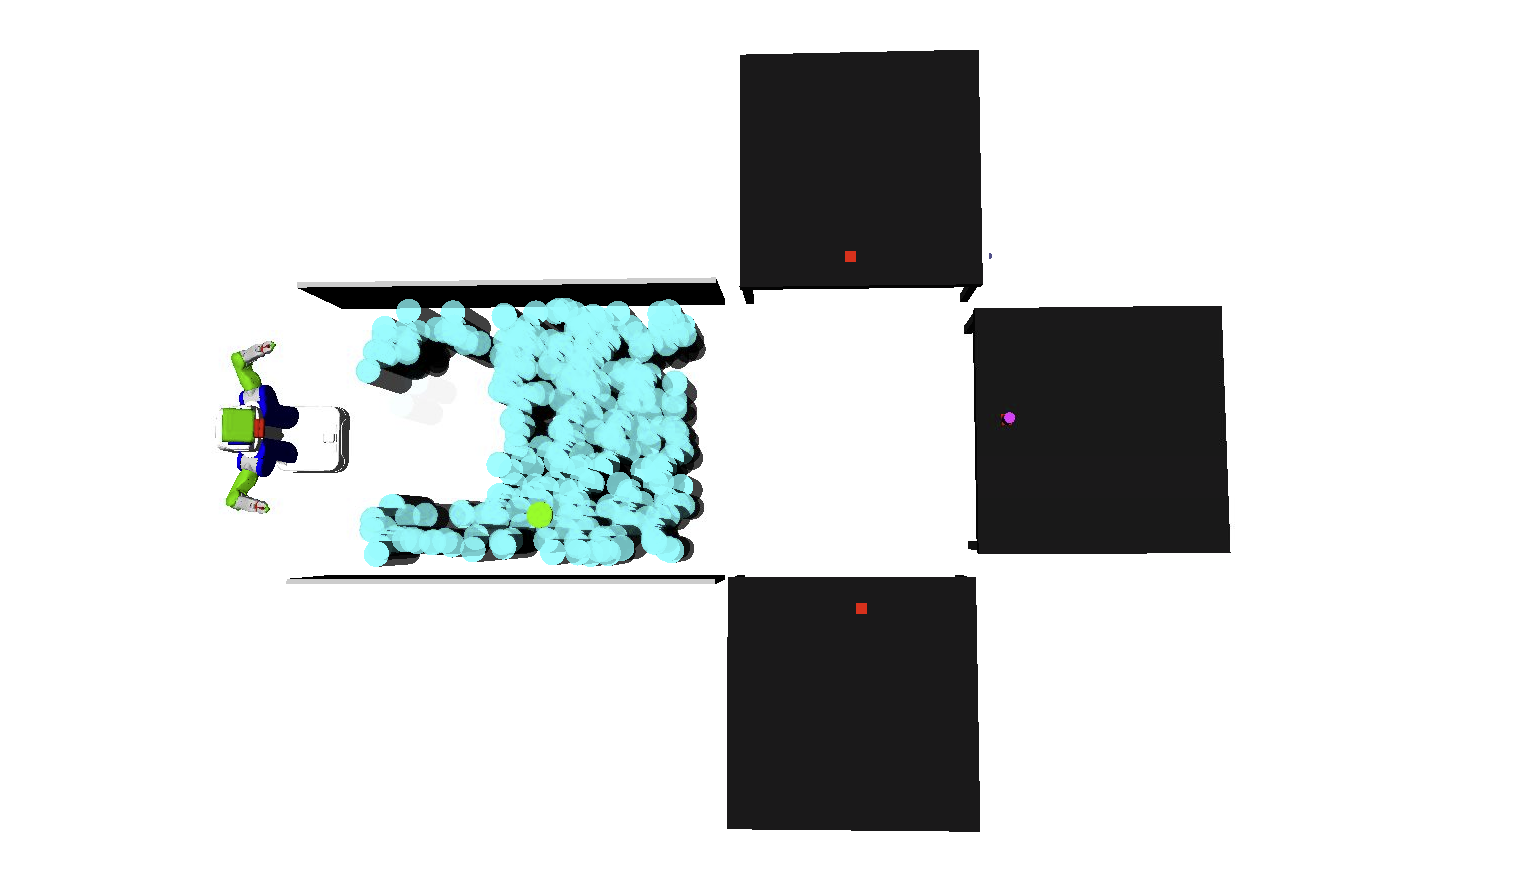
\includegraphics[width=\textwidth]{corridor_images/1-observe.png}
    \caption{After 1 observations}
  \end{subfigure}
  \begin{subfigure}[b]{0.22\linewidth}
    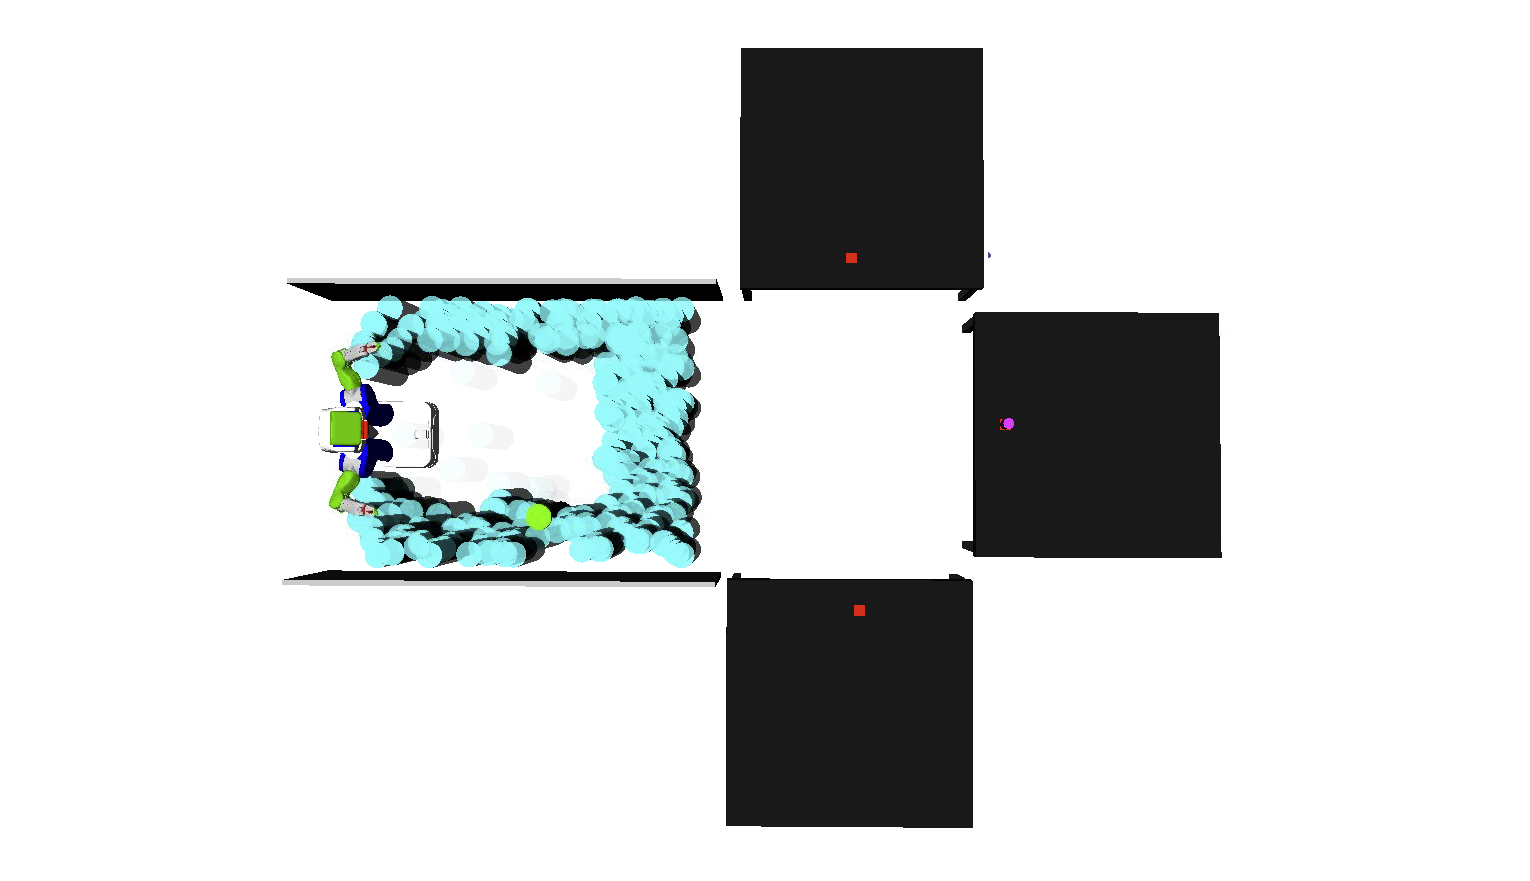
\includegraphics[width=\textwidth]{corridor_images/2-observe.png}
    \caption{After 2 observations}
  \end{subfigure}
  \begin{subfigure}[b]{0.22\linewidth}
    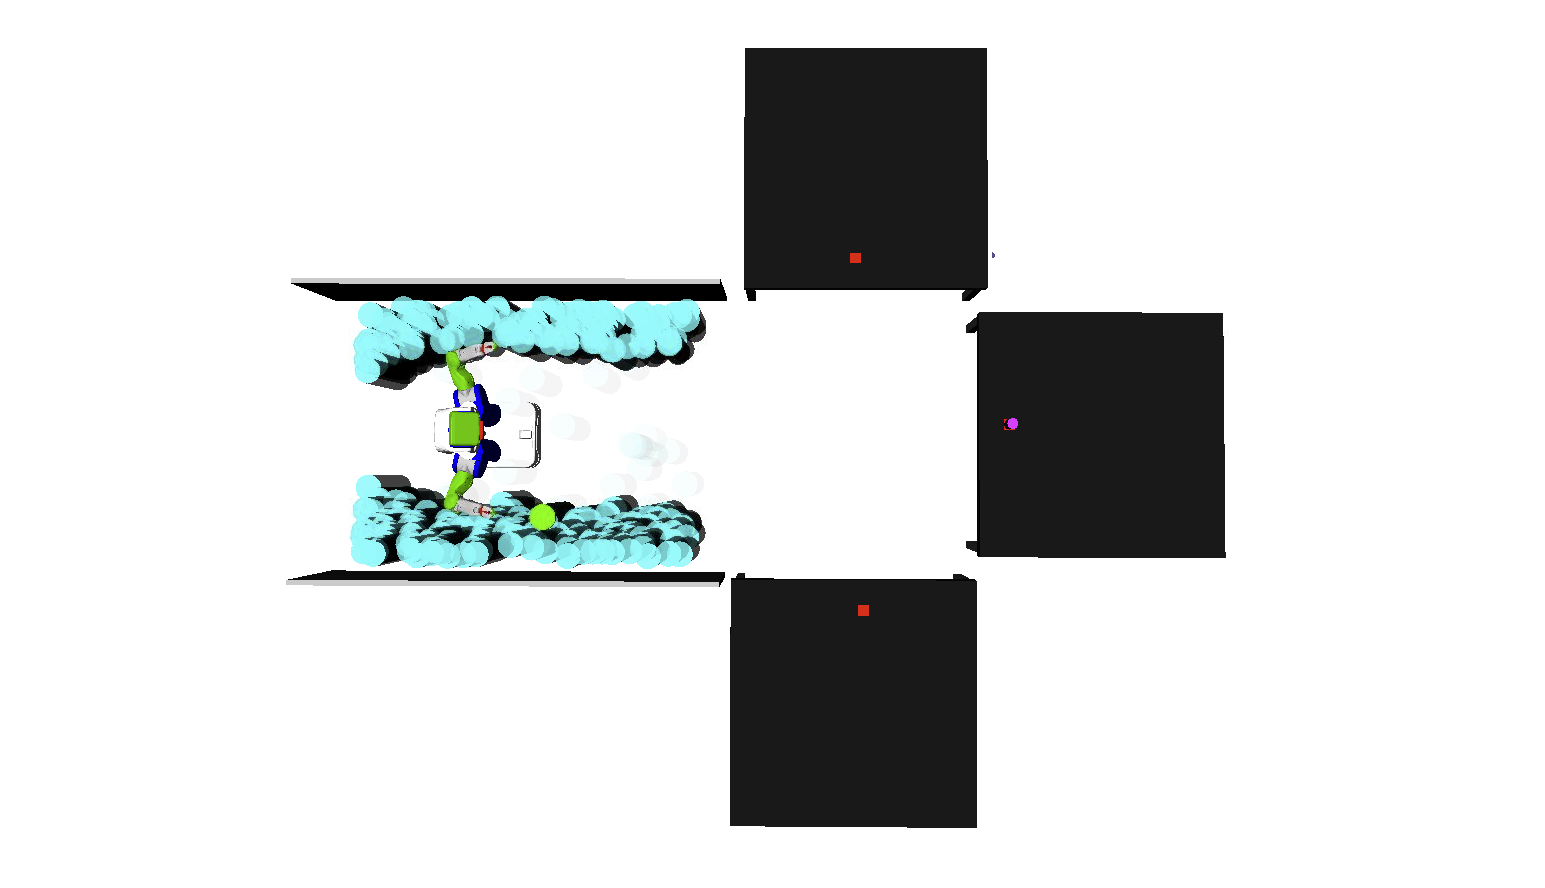
\includegraphics[width=\textwidth]{corridor_images/3-observe.png}
    \caption{After 3 observations}
  \end{subfigure}
  \caption{Execution trace of interfaced belief space planning
    traversing a corridor with uncertain obstacles.  The blue
    cylinders are drawn from a uniform prior distribution. After
    reaching the other side of the corridor, the robot will search for
    and pick up two target objects from the three tables.}
  \label{fig:corridorimgs}
\end{figure*}

We evaluate \ibsp{} in partially observable pick-and-place and navigation
tasks.  The robot in our simulation is a full model of the Willow
Garage PR2. We provide results for several prior distributions on
object locations: uni-modal Gaussian, multi-modal Gaussian, and uniform.
\subsection{Observation Operator Specification and Generators}
The maximum likelihood component of the determinized problem
essentially follows the dynamics specified in
\secref{sec-formulation}. In order to extend this domain to handle
partial observability, we add the following fluents and operators:
\begin{tightlist}
  \item[]Fluents: \\\emph{MLInView}(r\_pose, o\_pose\_bel)\\
    \emph{MLOccludes}(o, o\_pose\_bel, r\_obs\_pose)\\
    \emph{MLObstructs}(o, traj)\\
    \emph{UncertainGP}(o\_pose\_bel, r\_pose, grasp)\\
    \emph{UncertainObstructs}(o, traj)
  \item[]Operators:
  \begin{tightlist} \item \emph{ObserveGP}(r\_obs\_pose, o, o\_pose\_bel)
\begin{tightlist}
  \item[\emph{pre}:] \emph{MLLoc}(o, o\_pose\_bel) $\wedge$
    \emph{RLoc}(r\_obs\_pose) \\ $\wedge$
    \emph{MLInView}(r\_obs\_pose, o\_pose) \\ $\wedge$ $\forall o_i
    \lnot$\emph{MLOccludes}($o_i$, o\_pose\_bel, r\_obs\_pose)
  \item[\emph{eff}:] $\forall$ r\_p, g $\lnot$\emph{UncertainGP}(o\_pose\_bel, r\_p, g)
\end{tightlist}
\item  \emph{ObserveTrajectory}(r\_obs\_pose, traj) 

\begin{tightlist}
  \item[\emph{pre}:] \emph{RLoc}(r\_obs\_pose) \\$\wedge$
    \emph{MLInView}(r\_obs\_pose, traj)\\ $\wedge$
    $\forall o_i \lnot$\emph{MLOccludes}($o_i$, traj, r\_obs\_pose)
  \item[\emph{eff}:] $\forall o_i \lnot$\emph{UncertainObstructs}($o_i$,
    traj)
\end{tightlist}
\end{tightlist}
\end{tightlist}

The additional skolem functions needed to support this functionality
are \emph{ViewPose}(obj) and \emph{ViewPose}(traj) for object and
trajectory references. The generator for object view poses draws
samples from a 1-meter unit disc around the object, and the head pose
is fixed to point at the object's maximum likelihood position. The
generator for trajectory view poses returns the first step along the
trajectory that has non-negligible probability of being in
collision. To observe the uncertain step, a base pose is sampled from
regions with negligible collision probability along the same
trajectory.

\subsection{Observation model and state estimation}
In our experiments, we use an observation model that accounts for
false negatives, negative observations, and occlusion. We model our
sensor as a simulated head-mounted Kinect. We use ray-casting with
objects fixed to their maximum likelihood locations to build an
estimate of the visible region of the \mld{} for a given pose.

Under our model, we obtain false negatives in relation to the overlap
of the object with the visible region. We measure this overlap as the
ratio of penetration depth to the object radius. Penetration depth is
the minimum translation distance that removes the object from the
visible region and object radius is the radius of the smallest sphere
that encloses the object. This amounts to observing a false negative
with probability $1-\min \left( 1, \frac{\text{penetration
    depth}}{\text{object radius}} \right)$. If we do not get a false
negative, then we observe the object's pose with Gaussian noise.

In our domains, correctly accounting for negative observations is
critical: without them it is impossible to guarantee that a trajectory
is safe without first localizing all objects it could collide with. To
account for this, we use a factored representation of the belief
state. For each object we maintain an explicit posterior distribution
over its position (e.g., Kalman filter) that summarizes positive
observations and a set of view cones where it was not observed that
summarizes negative observations. We refer to the first component as
the positive observation distribution and the second as the negative
regions. 

Likelihood queries in this model are relatively straightforward. We
implement sampling with probabilistic rejection sampling: we sample
from the positive observation distribution and discard the sample with
probability proportional to the corresponding observation
likelihood. We answer maximum likelihood queries by sampling
repeatedly and returning the sample with maximum likelihood.

\subsection{Evaluations}
We implement our experiments in Python and use
OpenRave~\cite{Diankov_2008_6117} to represent the environment. We use
trajectory optimization for our motion
planning~\cite{schulman2013finding} and implement custom collision
checking in Flexible Collision Library~\cite{jia2014fcl}. We use the
Fast-Forward~\cite{FF} and Fast-Downward~\cite{helmert2006fast} task
planners to solve our high-level planning problems. Experiments were
run in series on Intel Core i7-4770K machines with 16GB RAM. We
validate our approach in three distinct scenarios.

To explore collision avoidance in robot navigation tasks under
uncertainty, we evaluate performance in a corridor domain. We place
the robot at one end of a corridor and present it with the goal of
finding and grasping objects on the other end of the corridor.  A
solution in this domain traverses the corridor observing at regular
intervals to ensure collision avoidance. Uniform distributions model
the locations of a varying number of obstructing columns throughout
the corridor. This task would be essentially insoluble
without a proper accounting of negative observations.

The second task demonstrates the ability for our system to reason
about occlusions. We set a goal of grasping a target object from a
cluttered table with other objects on it: some have deterministic
locations and others have a Gaussian prior distribution on their
location. The target object's location is also drawn from a Gaussian
distribution. \ibsp{} plans to remove any occlusions, observe the
target object, and then pick it up. In our experiments, 3 of the
objects on the table have unobserved locations.

Our final scenario illustrates planning under a multi-modal initial
state distribution. The robot has lost its keys and is trying to
locate them among three drawers they could be in.  We use a mixture of
Gaussians as the prior for the target's location. Each drawer that
could contain the object is obstructed from being fully opened by a
deterministic object. \ibsp{} begins by assuming the target is placed
at its maximum likelihood location. It discovers that the target is
occluded by the drawer containing it and plans to open this drawer. If
the drawer obstruction impedes the drawer from opening far enough for
the maximum likelihood observation to be useful, this obstruction fact
is also discovered and accounted for. During execution, we perform an
observation of the interior of the drawer. If the object is observed
we continue with the existing plan and achieve our goal. If it is not,
our system chooses to replan, as the negative observation indicates
the object is in a different drawer.

Table \ref{table:results} shows timing results for the three described
tasks. \figref{fig:drawerimgs} and \figref{fig:corridorimgs} show
intermediate steps and belief states for the drawer and corridor
tasks. The supplementary video demonstrates plan execution for all
three tasks.

\begin{table}
  \centering
  \vspace{8pt}
  \tabcolsep=0.11cm{
  \begin{tabular}{cccc}
    \toprule
      Problem Type & \% Solved & Avg Time (s) & Avg \# Planner Runs\\
    \midrule
      Uni. corridor, 1 obj & 100 & 232 & 1.88\\
    \midrule
      Uni. corridor, 2 obj & 100 & 445 & 2.45\\
    \midrule
      Uni. corridor, 3 obj & 88 & 926 & 2.78\\
    \midrule
      Uni. corridor, 4 obj & 58 & 1168 & 2\\
    \midrule
      Table, 5 obj & 95 & 89 & 2.2\\
    \midrule
      Table, 10 obj & 95 & 162 & 2.21\\
    \midrule
      Table, 15 obj & 83 & 135 & 2.26\\
    \midrule
      Table, 20 obj & 70 & 229 & 2.03\\
    \midrule
      Table, 25 obj & 68 & 166 & 1.84\\
    \midrule
      Table, 30 obj & 48 & 122 & 1.96\\
    \midrule
      3-drawer search & 93 & 325 & 2.11\\
    \bottomrule
  \end{tabular}}
  \caption{Solution percentages, running times, and number of
    high-level planner calls for \ibsp{} in occluded search and
    navigation tasks. `Uni. corridor $N$ obj' refers to our corridor
    navigation task with $N$ obstructions. `Table, $N$ obj' is the
    cluttered table task with $N$ objects on the table. `3-drawer
    search' is the multi-modal search problem. Results are averaged
    across 30 independent runs. Planning runs timeout after 1800s.}
  \label{table:results}
\end{table}



